\documentclass[11pt,addpoints]{exam}
\usepackage{fullpage}
\usepackage{amsfonts, amsmath, amssymb, amsthm}
\usepackage{mathtools}
\usepackage{enumerate}
\usepackage{listings}
\usepackage[boxed]{algorithm}
\usepackage[noend]{algpseudocode}
\algrenewcommand\algorithmicrequire{\textbf{Input:}}
\algrenewcommand\algorithmicensure{\textbf{Output:}}
\usepackage{hyperref}
\usepackage{tikz}
\usepackage[inline,shortlabels]{enumitem}
\usetikzlibrary{automata, positioning, arrows}
\usepackage{subcaption}


% in order to compile this file you need to get 'header.tex' from
% Canvas and change the line below to the appropriate file path
%%% theorems

\theoremstyle{plain}            % following are "theorem" style
\newtheorem{theorem}{Theorem}[section]
\newtheorem{lemma}[theorem]{Lemma}
\newtheorem{corollary}[theorem]{Corollary}
\newtheorem{proposition}[theorem]{Proposition}
\newtheorem{claim}[theorem]{Claim}
\newtheorem{fact}[theorem]{Fact}
\newtheorem{openproblem}[theorem]{Open Problem}

\theoremstyle{definition}       % following are def style
\newtheorem{definition}[theorem]{Definition}
\newtheorem{conjecture}[theorem]{Conjecture}
\newtheorem{example}[theorem]{Example}
\newtheorem{protocol}[theorem]{Protocol}
\newtheorem{exercise}[theorem]{Exercise}

\theoremstyle{remark}           % following are remark style
\newtheorem{remark}[theorem]{Remark}
\newtheorem{note}[theorem]{Note}
\newtheorem*{aside}{Aside}
\newtheorem*{gn}{Grading Note} % grading note

%%% special sets
\newcommand{\bit}{\ensuremath{\{0,1\}}}
\newcommand{\bitt}{\ensuremath{\{-1,1\}}}

% font for general-purpose algorithms
\newcommand{\algo}[1]{\ensuremath{\mathsf{#1}}}
% font for general-purpose computational problems
\newcommand{\problem}[1]{\ensuremath{\mathsf{#1}}}
% font for complexity classes
%\newcommand{\class}[1]{\ensuremath{\mathsf{#1}}}

\global\long\def\path{\mathrm{path}}
% asymptotics
%\DeclareMathOperator{\poly}{poly}
%\DeclareMathOperator{\polylog}{polylog}
\DeclareMathOperator{\negl}{negl}
\DeclareMathOperator{\Otil}{\tilde{O}}
\DeclareMathOperator{\Ostar}{O^*}

%%% "LEFT-RIGHT" PAIRS OF SYMBOLS

% inner product
\DeclarePairedDelimiter\inner{\langle}{\rangle}
% absolute value
\DeclarePairedDelimiter\abs{\lvert}{\rvert}
% a set
\DeclarePairedDelimiter\set{\{}{\}}
% parens
\DeclarePairedDelimiter\parens{(}{)}
% tuple, alias for parens
\DeclarePairedDelimiter\tuple{(}{)}
% square brackets
\DeclarePairedDelimiter\bracks{[}{]}
% rounding off
\DeclarePairedDelimiter\round{\lfloor}{\rceil}
% floor function
\DeclarePairedDelimiter\floor{\lfloor}{\rfloor}
% ceiling function
\DeclarePairedDelimiter\ceil{\lceil}{\rceil}
% length of some vector, element
\DeclarePairedDelimiter\length{\lVert}{\rVert}
% norm
\DeclarePairedDelimiter\norm{\lVert}{\rVert}
% length (as a string)
\DeclarePairedDelimiter\len{\lvert}{\rvert}
% bra-kets
\DeclarePairedDelimiter\bra{\langle}{\rvert}
\DeclarePairedDelimiter\ket{\lvert}{\rangle}
\newcommand{\braket}[2]{\ensuremath{\langle #1 \vert #2 \rangle}}
\newcommand{\ketbra}[2]{\ensuremath{\lvert #1 \rangle \langle #2 \rvert}}

%%% MATH OPERATORS
\DeclareMathOperator{\Var}{Var}
\DeclareMathOperator{\tr}{Tr}
\DeclareMathOperator{\supp}{supp}
\DeclareMathOperator{\var}{var}
\DeclareMathOperator{\vol}{vol}
\DeclareMathOperator{\sign}{sign}

%%% BLACKBOARD SYMBOLS

\newcommand{\C}{\ensuremath{\mathbb{C}}}
\newcommand{\D}{\ensuremath{\mathbb{D}}}
\newcommand{\F}{\ensuremath{\mathbb{F}}}
\newcommand{\G}{\ensuremath{\mathbb{G}}}
\newcommand{\J}{\ensuremath{\mathbb{J}}}
\newcommand{\N}{\ensuremath{\mathbb{N}}}
\newcommand{\Q}{\ensuremath{\mathbb{Q}}}
\newcommand{\R}{\ensuremath{\mathbb{R}}}
\newcommand{\T}{\ensuremath{\mathbb{T}}}
\newcommand{\Z}{\ensuremath{\mathbb{Z}}}
\newcommand{\QR}{\ensuremath{\mathbb{QR}}}

% sets in calligraphic type

\newcommand{\calD}{\ensuremath{\mathcal{D}}}
\newcommand{\calF}{\ensuremath{\mathcal{F}}}
\newcommand{\calG}{\ensuremath{\mathcal{G}}}
\newcommand{\calH}{\ensuremath{\mathcal{H}}}
\newcommand{\calI}{\ensuremath{\mathcal{I}}}
\newcommand{\calL}{\ensuremath{\mathcal{L}}}
\newcommand{\calN}{\ensuremath{\mathcal{N}}}
\newcommand{\calP}{\ensuremath{\mathcal{P}}}
\newcommand{\calS}{\ensuremath{\mathcal{S}}}
\newcommand{\calX}{\ensuremath{\mathcal{X}}}
\newcommand{\calY}{\ensuremath{\mathcal{Y}}}

% matrices and vectors

\newcommand{\matA}{\ensuremath{\mathbf{A}}}
\newcommand{\matB}{\ensuremath{\mathbf{B}}}
\newcommand{\matC}{\ensuremath{\mathbf{C}}}
\newcommand{\matD}{\ensuremath{\mathbf{D}}}
\newcommand{\matE}{\ensuremath{\mathbf{E}}}
\newcommand{\matF}{\ensuremath{\mathbf{F}}}
\newcommand{\matG}{\ensuremath{\mathbf{G}}}
\newcommand{\matH}{\ensuremath{\mathbf{H}}}
\newcommand{\matI}{\ensuremath{\mathbf{I}}}
\newcommand{\matJ}{\ensuremath{\mathbf{J}}}
\newcommand{\matK}{\ensuremath{\mathbf{K}}}
\newcommand{\matL}{\ensuremath{\mathbf{L}}}
\newcommand{\matM}{\ensuremath{\mathbf{M}}}
\newcommand{\matN}{\ensuremath{\mathbf{N}}}
\newcommand{\matO}{\ensuremath{\mathbf{O}}}
\newcommand{\matP}{\ensuremath{\mathbf{P}}}
\newcommand{\matQ}{\ensuremath{\mathbf{Q}}}
\newcommand{\matR}{\ensuremath{\mathbf{R}}}
\newcommand{\matS}{\ensuremath{\mathbf{S}}}
\newcommand{\matT}{\ensuremath{\mathbf{T}}}
\newcommand{\matU}{\ensuremath{\mathbf{U}}}
\newcommand{\matV}{\ensuremath{\mathbf{V}}}
\newcommand{\matW}{\ensuremath{\mathbf{W}}}
\newcommand{\matX}{\ensuremath{\mathbf{X}}}
\newcommand{\matY}{\ensuremath{\mathbf{Y}}}
\newcommand{\matZ}{\ensuremath{\mathbf{Z}}}
\newcommand{\matzero}{\ensuremath{\mathbf{0}}}

\newcommand{\veca}{\ensuremath{\mathbf{a}}}
\newcommand{\vecb}{\ensuremath{\mathbf{b}}}
\newcommand{\vecc}{\ensuremath{\mathbf{c}}}
\newcommand{\vecd}{\ensuremath{\mathbf{d}}}
\newcommand{\vece}{\ensuremath{\mathbf{e}}}
\newcommand{\vecf}{\ensuremath{\mathbf{f}}}
\newcommand{\vecg}{\ensuremath{\mathbf{g}}}
\newcommand{\vech}{\ensuremath{\mathbf{h}}}
\newcommand{\veck}{\ensuremath{\mathbf{k}}}
\newcommand{\vecm}{\ensuremath{\mathbf{m}}}
\newcommand{\vecp}{\ensuremath{\mathbf{p}}}
\newcommand{\vecq}{\ensuremath{\mathbf{q}}}
\newcommand{\vecr}{\ensuremath{\mathbf{r}}}
\newcommand{\vecs}{\ensuremath{\mathbf{s}}}
\newcommand{\vect}{\ensuremath{\mathbf{t}}}
\newcommand{\vecu}{\ensuremath{\mathbf{u}}}
\newcommand{\vecv}{\ensuremath{\mathbf{v}}}
\newcommand{\vecw}{\ensuremath{\mathbf{w}}}
\newcommand{\vecx}{\ensuremath{\mathbf{x}}}
\newcommand{\vecy}{\ensuremath{\mathbf{y}}}
\newcommand{\vecz}{\ensuremath{\mathbf{z}}}
\newcommand{\veczero}{\ensuremath{\mathbf{0}}}
\newcommand{\vecone}{\ensuremath{\mathbf{1}}}

%%% misc

\newcommand{\eps}{\varepsilon}

%%% for homework and section notes

\newcommand{\commonheader}[2]{
    \pagestyle{headandfoot}
    \setlength{\headheight}{26pt}
    \setlength{\headsep}{16pt}

    \header
        {\small{\textbf{EECS 376: Foundations of Computer Science}} \\ \footnotesize{\textbf{University of Michigan, Spring 2024}}}
        {#1}
        {#2}

    \firstpageheadrule
    \runningheadrule

    \footer
        {}
        {\thepage}
        {}
}

\newcommand{\hwheader}{
    \commonheader
        {\Large \textbf{Homework \hwnum}}
        {\small \textbf{Due 8:00pm, \duedate\\ {\tiny(accepted until 9:59 pm, no credit after)}}}
}

\newcommand{\hwslnheader}{
    \commonheader
    	{}
        {\Large \textbf{Solutions to Homework \hwnum}}
    \printanswers
}

\newcommand{\notesheader}{
    \commonheader
    	{}
        {\Large \textbf{Discussion Notes \sectionnum}}
}

\newcommand{\practiceheader}{
    \commonheader
    	{}
        {\Large \textbf{Discussion Worksheet \sectionnum}}
}

\newcommand{\practiceslnheader}{
    \commonheader
    	{}
        {\Large \textbf{Solutions to Discussion Worksheet \sectionnum}}
}

\newcommand{\reviewheader}{
    \commonheader 
    \smallskip
    	{}
        {\Large \textbf{Midterm Review Notes}}
}

\newcommand{\hwpreface}{

\noindent This homework has \numquestions\ questions, for a total of \numpoints\ points and \numbonuspoints\ extra-credit points.

\noindent Unless otherwise stated, each question requires \emph{clear}, \emph{logically correct}, and \emph{sufficient} justification to convince the reader.

\noindent For bonus/extra-credit questions, we will provide very limited guidance in office hours and on Piazza, and we do not guarantee anything about the difficulty of these questions.
 
\noindent We strongly encourage you to typeset your solutions in \LaTeX.

\noindent If you collaborated with someone, you must state their name(s). You must \emph{write your own solution} for all problems and \emph{may not use any other student’s write-up}.
}

\newcommand{\hint}[1]{
\emph{Hint}: #1
}
\newcommand{\bonus}{
\emph{Optional bonus}:
}
\newcommand{\extracredit}{
\emph{Extra credit}: 
}


\newcommand{\hwnum}{5}
\newcommand{\duedate}{February 14}
\usepackage{xcolor}

\hwheader   % header for homework
% \hwslnheader   % header for homework solutions

% Comment the following line in order to hide solutions.
% Uncomment the line to show solutions written inside of
% LaTeX solution environments like:
% \begin{solution}
%   My solution.
% \end{solution}.
\printanswers

\begin{document}

\hwpreface

\pointsinmargin
\pointpoints{pt}{pts}
\bonuspointpoints{EC pt}{EC pts}
\marginpointname{ \points}
\marginbonuspointname{ \bonuspoints}

\begin{questions}
  \addtocounter{question}{-1}

  \question[0] \textbf{Before you start; before you submit.}
  
  If applicable, state the name(s) and uniqname(s) of your collaborator(s).

  \begin{solution}

  \end{solution}

  \question[10] \textbf{Self assessment.}
  
  Carefully read and understand the posted solutions to the previous homework; you may also find the video ``walkthroughs'' in the Canvas Media Gallery helpful.
  Identify one part for which your own solution has the most room for improvement (e.g., has unsound reasoning, doesn’t show what was required, could be significantly clearer or better organized, etc.).
  Copy or screenshot this solution, then in a few sentences, explain what was deficient and how it could be fixed.

  (Alternatively, if you think one of your solutions is significantly \emph{better} than the posted one, copy it here and explain why you think it is better.)

  If you didn't turn in the previous homework, then (1)~state that you didn't turn it in, and (2)~pick a problem that you think is particularly challenging from the previous homework, and explain the answer in your own words.
  You may reference the answer key, but your answer should be in your own words.

  \begin{solution}

  \end{solution}

  \question \textbf{Short answer.}

  \begin{parts}

    \part[4]
    Write the state-transition function (called~$\delta$ in the lecture and the notes) for the following DFA, as a table.
    Also give a regular expression (using the ``string notation'' from class) for the language this DFA decides.
    No justification is required for either of these.
    For reference on formatting the state-transition function, see the \href{https://eecs376.github.io/notes/computability.html#finite-automata}{lecture notes on Finite Automata}.

    \begin{center}
      \begin{tikzpicture}[scale=0.2]
        \tikzstyle{every node}+=[inner sep=0pt]
        \draw [black] (19.8,-24.9) circle (3);
        \draw (19.8,-24.9) node {$q_0$};
        \draw [black] (31.6,-24.9) circle (3);
        \draw (31.6,-24.9) node {$q_1$};
        \draw [black] (31.6,-24.9) circle (2.4);
        \draw [black] (42.5,-24.9) circle (3);
        \draw (42.5,-24.9) node {$q_2$};
        \draw [black] (31.6,-16) circle (3);
        \draw (31.6,-16) node {$q_3$};
        \draw [black] (22.8,-24.9) -- (28.6,-24.9);
        \fill [black] (28.6,-24.9) -- (27.8,-24.4) -- (27.8,-25.4);
        \draw (25.7,-25.4) node [below] {$1$};
        \draw [black] (34.6,-24.9) -- (39.5,-24.9);
        \fill [black] (39.5,-24.9) -- (38.7,-24.4) -- (38.7,-25.4);
        \draw (37.05,-25.4) node [below] {$0$};
        \draw [black] (21.811,-22.675) arc (135.15544:118.89448:31.429);
        \fill [black] (28.91,-17.32) -- (27.97,-17.27) -- (28.45,-18.15);
        \draw (24.16,-19.25) node [above] {$0$};
        \draw [black] (31.6,-21.9) -- (31.6,-19);
        \fill [black] (31.6,-19) -- (31.1,-19.8) -- (32.1,-19.8);
        \draw (31.1,-20.45) node [left] {$1$};
        \draw [black] (34.336,-17.226) arc (61.87063:39.66514:21.509);
        \fill [black] (34.34,-17.23) -- (34.81,-18.04) -- (35.28,-17.16);
        \draw (38.81,-19.04) node [above] {$0$};
        \draw [black] (30.277,-13.32) arc (234:-54:2.25);
        \draw (31.6,-8.75) node [above] {$0,1$};
        \fill [black] (32.92,-13.32) -- (33.8,-12.97) -- (32.99,-12.38);
        \draw [black] (41.275,-27.598) arc (-40.00598:-139.99402:5.516);
        \fill [black] (32.83,-27.6) -- (32.96,-28.53) -- (33.72,-27.89);
        \draw (37.05,-30.07) node [below] {$1$};
        \draw [black] (12.9,-24.9) -- (16.8,-24.9);
        \draw (12.4,-24.9) node [left] {$start$};
        \fill [black] (16.8,-24.9) -- (16,-24.4) -- (16,-25.4);
      \end{tikzpicture}
    \end{center}

    \begin{solution}

    \end{solution}

    \part[4] Give a regular expression (using the ``string notation'' from class) for the language decided by the following DFA.
    No justification is required.

    \begin{center}
      \begin{tikzpicture}[scale=0.2]
        \tikzstyle{every node}+=[inner sep=0pt]
        \draw [black] (17.1,-27.6) circle (3);
        \draw (17.1,-27.6) node {$q_0$};
        \draw [black] (30.5,-27.6) circle (3);
        \draw (30.5,-27.6) node {$q_1$};
        \draw [black] (45.1,-27.6) circle (3);
        \draw (45.1,-27.6) node {$q_2$};
        \draw [black] (61.1,-27.6) circle (3);
        \draw (61.1,-27.6) node {$q_3$};
        \draw [black] (27.3,-42.8) circle (3);
        \draw (27.3,-42.8) node {$q_4$};
        \draw [black] (45.1,-42.8) circle (3);
        \draw (45.1,-42.8) node {$q_5$};
        \draw [black] (61.1,-42.8) circle (3);
        \draw (61.1,-42.8) node {$q_6$};
        \draw [black] (61.1,-42.8) circle (2.4);
        \draw [black] (9,-27.6) -- (14.1,-27.6);
        \draw (8.5,-27.6) node [left] {$start$};
        \fill [black] (14.1,-27.6) -- (13.3,-27.1) -- (13.3,-28.1);
        \draw [black] (20.1,-27.6) -- (27.5,-27.6);
        \fill [black] (27.5,-27.6) -- (26.7,-27.1) -- (26.7,-28.1);
        \draw (23.8,-27.1) node [above] {$b$};
        \draw [black] (29.177,-24.92) arc (234:-54:2.25);
        \draw (30.5,-20.35) node [above] {$a$};
        \fill [black] (31.82,-24.92) -- (32.7,-24.57) -- (31.89,-23.98);
        \draw [black] (33.5,-27.6) -- (42.1,-27.6);
        \fill [black] (42.1,-27.6) -- (41.3,-27.1) -- (41.3,-28.1);
        \draw (37.8,-27.1) node [above] {$b$};
        \draw [black] (25.202,-40.656) arc (-137.66799:-154.60463:42.126);
        \fill [black] (25.2,-40.66) -- (25.03,-39.73) -- (24.29,-40.4);
        \draw (20.76,-37.1) node [left] {$a$};
        \draw [black] (26.632,-45.713) arc (14.80554:-273.19446:2.25);
        \draw (21.33,-48.53) node [below] {$a,b$};
        \fill [black] (24.58,-44.04) -- (23.68,-43.76) -- (23.94,-44.73);
        \draw [black] (48.1,-27.6) -- (58.1,-27.6);
        \fill [black] (58.1,-27.6) -- (57.3,-27.1) -- (57.3,-28.1);
        \draw (53.1,-27.1) node [above] {$a$};
        \draw [black] (59.777,-24.92) arc (234:-54:2.25);
        \draw (61.1,-20.35) node [above] {$b$};
        \fill [black] (62.42,-24.92) -- (63.3,-24.57) -- (62.49,-23.98);
        \draw [black] (61.1,-30.6) -- (61.1,-39.8);
        \fill [black] (61.1,-39.8) -- (61.6,-39) -- (60.6,-39);
        \draw (61.6,-35.2) node [right] {$a$};
        \draw [black] (42.42,-44.123) arc (-36:-324:2.25);
        \draw (37.85,-42.8) node [left] {$b$};
        \fill [black] (42.42,-41.48) -- (42.07,-40.6) -- (41.48,-41.41);
        \draw [black] (48.1,-42.8) -- (58.1,-42.8);
        \fill [black] (58.1,-42.8) -- (57.3,-42.3) -- (57.3,-43.3);
        \draw (53.1,-42.3) node [above] {$a$};
        \draw [black] (58.632,-44.503) arc (-58.51014:-121.48986:27.629);
        \fill [black] (29.77,-44.5) -- (30.19,-45.35) -- (30.71,-44.49);
        \draw (44.2,-49.07) node [below] {$a,b$};
        \draw [black] (45.1,-30.6) -- (45.1,-39.8);
        \fill [black] (45.1,-39.8) -- (45.6,-39) -- (44.6,-39);
        \draw (44.6,-35.2) node [left] {$b$};
      \end{tikzpicture}
    \end{center}
    
    \begin{solution}

    \end{solution}


    \part[4] Consider the following claim: a minimum spanning tree in a graph is \emph{unique} if the edge weights are \emph{distinct} (all different).

    Briefly explain what is wrong with the following bogus ``proof'' of this claim: \emph{because edge weights are distinct, all choices in Kruskal's algorithm are completely determined---there are no ``ties'' between edge weights that the algorithm can choose how to break.
      So, the algorithm has only one possible output.
      Because Kruskal's algorithm is correct for the MST problem, its unique output must be the only minimum spanning tree in the graph.}

    \begin{solution}

    \end{solution}

    \part[4] 
    Give a correct proof for the claim in the previous part.

    \begin{solution}

    \end{solution}
  \end{parts}

  \question \textbf{Greedy knapsack filling.}

  Recall that in the ``0-1'' knapsack problem, you are given~$n$ items, where the $i$th item has weight~$w_{i}$ and value~$v_{i}$ (both positive), and a non-negative weight capacity~$C$ of the knapsack.
  An optimal solution is a subset $S\subseteq \set{1, 2, \ldots, n}$ of the items having maximum total value \[ \sum_{i\in S} v_i \; \text, \] under the constraint that the total weight is at most the knapsack capacity, i.e., \[ \sum_{i\in S} w_i \leq C \; \text. \]

  In this problem, we introduce the \emph{fractional} variant of the knapsack problem, where one may take any fraction $p_i \in [0,1]$ of any item~$i$.
  Naturally, a $p_i$-fraction of item~$i$ weighs $p_i \cdot w_i$, and has value $p_i \cdot v_i$.
  The goal is to maximize the total value of the selected fractional items.

  \begin{parts}

    \part[3] 
    Briefly explain why the optimal value for the fractional knapsack problem is \emph{at least as large} as that of the original 0-1 knapsack problem (for the same weights, values, and knapsack capacity).

    \begin{solution}

    \end{solution}
    
    \part[4] Consider the following two greedy algorithms for the fractional knapsack problem:
    \begin{itemize}
    \item Algorithm $A$: While there is still some unused knapsack capacity, choose an item having the \emph{largest value} (among those not considered yet), and add the largest possible fraction of that item (up to the entire item) that will fit within the remaining knapsack capacity.
      
    \item Algorithm $B$: While there is still some unused knapsack capacity, choose an item having the \emph{smallest weight} (among those not considered yet), and add the largest possible fraction of that item (up to the entire item) that will fit within the remaining knapsack capacity.
    \end{itemize}

    Suppose we run \emph{both} algorithms $A$ and $B$, and output a best one of their two outputs.
    Is this a correct algorithm for the fractional knapsack problem?
    If so, prove it.
    Otherwise, give an input for which this algorithm's output is not optimal, and show why it is not.

    \begin{solution}

    \end{solution}

    \part[7] Consider the following greedy algorithm for the fractional knapsack problem:
    \begin{itemize}
    \item Algorithm $C$: While there is still some unused knapsack capacity, choose an item having the largest \emph{relative value} $v_i/w_i$ (among those not considered yet), and add the largest possible fraction of that item (up to the full item) that will fit within the remaining knapsack capacity.
    \end{itemize}
    
    Here is the skeleton of an inductive proof that Algorithm $C$ outputs an optimal solution.
    Without loss of generality, suppose that the items are in sorted order by relative value $r_{i}=v_{i}/w_{i}$, from largest to smallest (the algorithm considers them in this order).
    View any selection of fractional items as a sequence $p_{1}, p_{2}, \ldots, p_{n}$, where $p_i$ is the fraction of item~$i$.
    Let $g_1, g_2, \ldots, g_n$ be the sequence of fractions that the greedy algorithm selects.
    We aim to prove the following claim:
    \begin{quote}
      For \emph{every} $k=0, \ldots, n$, the first~$k$ values $g_{1}, \ldots, g_{k}$ of this sequence are a prefix of (i.e., are the first~$k$ item fractions in) \emph{some} optimal solution. 
    \end{quote}
    Given this claim, the full sequence (for $k=n$) is itself an optimal solution, because there are no more items that can be (fractionally) selected.

    Prove the claim by induction.
    Specifically, establish the base case $k=0$, and then prove the inductive step, which says: for any $k < n$, if $g_{1}, \ldots, g_{k}$ is a prefix of \emph{some} optimal solution $OPT = o_{1}, \ldots, o_{n}$, then $g_{1}, \ldots, g_{k}, g_{k+1}$ is a prefix of \emph{some} optimal solution $OPT' = o'_{1}, \ldots, o'_{n}$.
    Use an exchange argument to modify $OPT$ into a valid selection $OPT'$, without reducing the value (so that it remains optimal).

    \begin{solution}

    \end{solution}

    \part[8] Now consider a new variant of the fractional knapsack problem, in which there are~$\ell$ knapsacks, where the $j$th knapsack has capacity $C_j$, and we aim to maximize the total value across all the knapsacks.
    Give a greedy algorithm that solves this variant.
    
    \begin{solution}

    \end{solution}
  \end{parts}

  \question \textbf{Greedy touring.}

  PETROBLUE, in support of the M Bus Formula One Team, has innovated a modular fuel pack for a bus that will transport EECS 376 students on a tour through various towns in Michigan.
  This fuel pack allows the vehicle to travel a certain distance before refueling.
  Each town has a service station where a fuel pack can be reloaded: the current pack is simply swapped out for a fresh full one.
  (Any remaining fuel in the removed pack will not be used by the bus.)
  The goal is to visit the towns in a specified order, while minimizing the number of fuel pack reloads.

  We model this problem as follows.
  The bus can travel a distance up to~$R$ on a single fuel pack.
  There are~$n$ towns to visit in sequence.
  For $i=1, \ldots, n$, the distance from the $(i-1)$st town (or from the starting point, when $i=1$) to the $i$th town is $d_i \leq R$.
  Given~$R$ and an array $D[1,\ldots,n] = [d_1, \ldots, d_n]$ as input, the goal is to find a \emph{smallest} set $S \subseteq \set{1,\ldots,n}$ of towns (specified by their indices) where refueling should occur, so that the bus can reach all~$n$ towns without running out of fuel at any point.
  The bus starts out with a full fuel pack, and no refueling is needed at the final town.

  \begin{parts}

    \part[8] Give a greedy algorithm (including pseuodocode) that solves this problem.
    Defer a correctness argument to the next part, but provide everything else involved in ``giving an algorithm'' here.
    
    \begin{solution}

    \end{solution}
    
    \part[8] Give an inductive proof using an exchange argument (like the ones presented in lecture and in the previous problem) that your algorithm from the previous part is correct.
    
    \begin{solution}

    \end{solution}
    
    \part[4] Now, suppose that the price of a fuel pack may differ from town to town.
    For example, a fuel pack might cost \$8 in the first town, \$3 in the second town, etc.
    So, the input now also includes an array $C=[c_1, \ldots, c_n]$, where~$c_i$ is the cost of refueling in the $i$th town.
    The goal now is to complete the tour while \emph{minimizing the total cost} of the fuel packs that are purchased along the way.

    PETROBLUE claims that we should use the same greedy algorithm that you proposed above to solve this problem.
    Determine whether this claim is true or not.
    If it is, give a proof.
    Otherwise, provide a small counterexample: give a specific input, the output of your greedy algorithm on that input, and a better solution for that input; also, \emph{very briefly} explain where your proof from the previous part fails for this problem.

    \begin{solution}

    \end{solution}
    
    \bonuspart[3] \emph{Optional extra credit.}
    Give an efficient dynamic programming algorithm (with recurrence and bottom-up implementation) that solves the problem from the previous part.
    
    \begin{solution}
    \end{solution}
  \end{parts}

  \question \textbf{Selecting suitable skis.}

  Suppose there are~$n$ skiers of various heights, and~$n$ pairs of skis having various lengths.
  (Both skis in a pair have the same length.)
  We want to match each skier with a pair of skis so as \emph{minimize the total difference} between each skier's height and the length of their skis.

  Formally, we are given a \emph{sorted} array $P[1,\ldots,n]$ of the skiers' heights (where $P[i] \leq P[i+1]$ for all $i<n$), and a (not necessarily sorted) array $S[1,\ldots,n]$ of the skis' lengths.
  We want to return a rearrangement (permutation) $S'[1,\ldots,n]$ of~$S$ that minimizes \[ \sum_{i=1}^n \abs*{ P[i] - S'[i] } \text. \]

  \begin{parts}
    \part[3] Give an $O(1)$-time algorithm for the case $n=2$.
    
    \begin{solution}

    \end{solution}
    
    \part[7] For general~$n$, consider an algorithm that just returns $S$ in sorted order.
    We can view this as a greedy algorithm that just repeatedly selects a pair of skis of shortest length (among those that remain).
    So, it makes exactly~$n$ selections $s'_1, s'_2, \ldots, s'_n$ in sorted order.
    
    Give an inductive proof using an exchange argument (like the ones presented in lecture and in the previous problems) that this algorithm is correct.

    \hint{Use the previous part as an ingredient of your proof.}
    
    \begin{solution}

    \end{solution}
  \end{parts}

  \question \textbf{Decision problems and languages.}

  Recall that the goal of a \emph{decision problem} is to determine whether a given input ``object'' has a certain ``property'', e.g., determine whether a given integer is prime, or whether a given string is a palindrome.
  In class, we said that any decision problem is equivalent to a \emph{membership problem} for a corresponding \emph{language}.
  That is, determining whether a given object has the property is equivalent to determining whether its encoding (as a string) is a member of the language.

  For each of the following decision problems, (i)~define a reasonable (finite) alphabet~$\Sigma$, (ii)~give the encoding (over the alphabet) of a representative input object, (iii)~analyze the length of the encoding in terms of the value of the input, and (iv) define a language~$L$ for the corresponding decision problem.
  Use the notation~$\inner{X}$ for the encoding of object~$X$ as a string over the alphabet.
  As examples, we have provided solutions to the first two parts.
  
  \begin{parts}
    \part[0] ``Does a given non-negative integer $k$ have 3 as its last digit, when written in base 10?''
    
    \begin{solution}
      \begin{enumerate}[(i)]
      \item A reasonable alphabet consists of the decimal digits, $\Sigma = \set{\texttt{0}, \ldots, \texttt{9}}$.

      \item Encoding: for an integer $k$, write it in base 10 in the usual way, as a string of digits.
        For example, if $k$ is the integer forty-seven, then $\langle k \rangle = \texttt{47}$.
        We stress that this is a \emph{string} of the characters \texttt{4} and \texttt{7}, which \emph{represents} the number forty-seven.

      \item The length of this encoding would be the number of digits in the value, which is $\Theta(\log k)$.

      \item A corresponding language would be $L_{EndsWith3} = \set{\langle k \rangle : k \bmod 10 = 3}$.
        It would also be acceptable to copy the phrasing of the decision problem, i.e., $L_{EndsWith3} = \set{\langle k \rangle : k \text{ written in base 10 has 3 as the last digit}}$
      \end{enumerate}

      Alternatively, we could also encode integers in binary, using the alphabet $\Sigma=\set{0,1}$.
      For example, if $k=5$, then $\langle k \rangle = \texttt{101}$.
      The length of this encoding is still $\Theta (\log k)$.
      The above two definitions of the language hold without modification, because they both describe membership only in terms of the \emph{value} of~$k$, not its encoding.
    \end{solution}
    
    \part[0] ``Is a given array of non-negative integers sorted?''
    
    \begin{solution}
      \begin{enumerate}[(i)]
      \item A reasonable alphabet $\Sigma$ is the set of ASCII characters, or more selectively, the decimal digits along with some separator characters: $\Sigma = \set{\texttt{0}, \ldots, \texttt{9}, \texttt{[}, \texttt{,}, \texttt{]}}$.
        (Notice that a comma is one of these characters.)

        Note: we can't just use the decimal digits alone if we want to use some special symbols to indicate the start/end of the array and to separate the elements.
        
      \item Example encoding: For an array $A$, encode its elements as in the previous part, and list those encodings with appropriate separators.
        For example, the array $A$ with entries one, two, three, and four would have $\langle A \rangle = \texttt{[1,3,2,4]}$.
      \item The length of this encoding is $\Theta(n + e)$, where~$n$ is the number of elements in the array, and $e$ is the total length of the encoding of the elements.
      \item The corresponding language is \[ L_{sorted} = \set{\langle A \rangle : A \text{ is a sorted array of non-negative integers.}}. \]
      \end{enumerate}
    \end{solution}
    
    \part[3] ``Given an array~$S$ of integers, are all its elements distinct?''
    
    \begin{solution}

    \end{solution}
    
    \part[3] ``Is a given undirected graph complete?''
    \hint{Consider the adjacency matrix.}
    
    \begin{solution}

    \end{solution}
    
    \part[3] ``Does a given C++ program halt when run on a given input?''

    \begin{solution}

    \end{solution}
  \end{parts}

  \question \textbf{Deciding languages with DFAs.}

  For each of the following languages, give a DFA that decides it.
  You may represent a DFA as a state-transition function or as a diagram, whichever you prefer.

  \begin{parts}
    \part[3] The language (over alphabet $\set{a,b}$) corresponding to the regular expression $ab^*$ .

    \begin{solution}

    \end{solution}

    \part[5] The language (over alphabet $\set{a,b}$) corresponding to the regular expression $b(aaa)^*b$.

    \begin{solution}

    \end{solution}

    \part[5]
    The language of binary strings in which the number of $0$s is divisible by 3 \emph{and} the number of $1$s is even.
    
    For example, the strings $\varepsilon$, $000$, $01010$, and $11000$ are in this language, while $1$, $01$, $001$, $0011$, and $000111$ are not.
    
    \begin{solution}

    \end{solution}
    
    \bonuspart[4] \emph{Optional extra credit.}
    
    Consider the following language: 
    \[ L=\set{x \in \{0,1\}^* : [ x ] \bmod 3 = 0}.
    \] where $[ x ] := \sum_{i=0}^n 2^{i} x_i$ for $x = x_0x_1\ldots x_n$.
    E.g., $[ \varepsilon ] = 0$ and $[ 01100000 ] = [ 011 ] = 6$.
    Note that the bits are given in `reverse' order from what is typical (e.g., 6 in binary is usually written as 110).

    Give a DFA that decides the language $L$.

    \hint{Relate $[ x_0x_1\ldots x_{k} ]$ to $[ x_0x_1\ldots x_{k-1} ]$, $x_k$, and~$k$.
      You can use the fact (which is easy to prove) that $2^{2m} \bmod 3 = 1$ and $2^{2m+1} \bmod 3 = 2$ for any non-negative integer~$m$.}
    
    \begin{solution}

    \end{solution}
  \end{parts}

  \bonusquestion[3] \emph{Optional extra credit.}
  \newcommand{\open}{\texttt{(}}
  \newcommand{\close}{\texttt{)}}

  Consider the alphabet $\Sigma = \set{\open,\close}$, which consists of the open- and close-parenthesis characters \open{} and \close{}.
  Say that a string $x \in \Sigma^*$ is \emph{balanced} if~$x$ has an equal number of \open{} and \close{} characters, and every \emph{prefix} of~$x$ has at least as many \open{} characters as \close{} ones.

  For example, the empty string $\varepsilon$, \open{}\open{}\close{}\open{}\close{}\close{}, and \open{}\open{}\open{}\close{}\close{}\close{} are balanced, but \open{}\close{}\close{}\open{}\open{}\close{} is not, because it fails the second condition (but not the first one).

  Either give a DFA that decides the language of balanced strings over $\Sigma$, or rigorously prove that no such DFA exists.

  \begin{solution}

  \end{solution}
\end{questions}

\end{document}